\subsection{Datenspeicherung}
\label{subsec:Datenspeicherung}
Während des Projekt 5 wurde die Datenspeicherung bereits mittels Breakout Board im Prototyp implementiert. Nachfolgend wird die Dokumentation aus dem Fachbericht des Projekt 5 übernommen und in einem weiteren Abschnitt Ergänzungen dazu aus der Bachelor-Thesis erläutert.

\subsubsection{Datenspeicherung - Projekt 5}
Die Datenspeicherung beinhaltet die gespeicherten Messwerte der Sensoren. Die Daten werden dann in einem *.txt-File nicht flüchtig gespeichert. Bei Beschädigung der Hardware können dann die zuletzt erfassten Daten immer noch mittels eines SD-Karten-Adapters von einem Computer ausgelesen werden. Als Kommunikationsprotokoll für das Schreiben und Auslesen der Karte wird SPI verwendet.

\subsubsection*{$\mu$SD-Karte}
\begin{minipage}{0.44\textwidth}
\centering
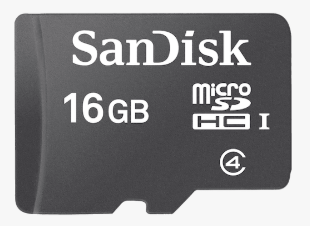
\includegraphics[width=0.4\textwidth]{graphics/Datenspeicherung/micro_sd_card_16GB.png}
\captionof{figure}{16 GB $\mu$SD-Karte \cite{musdkarte}}
\label{fig:muSDKarte}
\end{minipage}
\begin{minipage}{0.55\textwidth}
Bei der $\mu$SD-Karte muss auf die Kompatibilität mit dem Breakoutboard geachtet werden. Dafür sind folgende Kriterien zu beachten:\\
\begin{itemize}
\item Die $\mu$SD-Karte muss FAT16 oder FAT 32 formatiert sein.
\item Es sind nur die SD und SD High Capacity (SDHC) kompatibel.\\
\end{itemize}
\end{minipage}
Für die Umsetzung dieses Projektes wurde eine $\mu$SD-Karte der SD-Familie SDHC \Romannum{1} verwendet (siehe Abb. \ref{fig:muSDKarte}). SDHC sind Kapazitäten bis zu 32GB möglich und FAT32 formatiert. \cite{muSDspez}\\ 
Die Grösse eines Strings lässt sich nach der Gleichung \ref{equ:berechnung_stringgroesse} berechnen, wenn angenommen wird, dass jeder Buchstaben (char) 8 Bit hat und zum Schluss noch ein Terminator für das Stringende angehängt wird:
\begin{equation}
\centering
Anzahl\ Zeichen * 1\ Byte + 1 = String\ Grösse\ in\ Byte
\label{equ:berechnung_stringgroesse}
\end{equation}
Bei einer Speicherung der Daten nach der Struktur in Abb. \ref{fig:datenausgabe} würden somit leicht aufgerundet ca. 216 Byte pro Speichersatz benötigt werden.\\
\todo{Kontrolle ref fig:datenausgabe}
Da momentan eine 16GB grosse $\mu$SD-Karte verwendet wird, ergeben sich daraus
\begin{equation}
\dfrac{16E9}{216}=74.1E6 \approx \underline{\underline{74E6}}
\end{equation}
Speichersätze. Würden in einem zehn Minuten Zeitintervall ein Speichersatz abgespeichert werden, dann könnten 1411 Jahre 40 Wochen 4 Tage 21 Stunden 20 Minuten lang Werte von der Wetterstation abgespeichert werden. Diese Anzahl könnte noch verdoppelt werden, da wie oben bereits erwähnt $\mu$SD-Karten bis zu 32GB kompatibel sind.\\
\newpage
\subsubsection{Ergänzungen aus der Bachelor-Thesis}
Im Gegensatz zum Prototyping wird für die endgültige Wetterstation kein Breakout Board mehr verwendet. Die $\mu$SD-Karte wird in ein $\mu$SD-Karten-Adapter (Speicherkartenverbinder) gesteckt, welcher über ein Buffer (74HC4050) mit der MCU verbunden ist (siehe Abbildung \ref{fig:Uebersicht_PCB_MCU_RTC_SD_Sense}). Der 74HC4050 kann als Levelshifter verwendet werden und als Treiber für kapazitive Ladungen. In unserem Fall werden MCU und Speicherkartenverbinder mit 3.3V betrieben, weshalb kein Levelshifter notwendig ist. Der 74HC4050 wird demnach bei der Wetterstation als Treiber für kapazitive Ladungen verwendet.\\

Die Daten werden mit der Sensorik ermittelt, über die MCU verarbeitet und in der $\mu$SD-Karte gespeichert. Nun sollen die Daten jedoch per SMS (GSM) abrufbar sein und die Wetterstation ebenfalls über ein GPS-Modul verfügen. Aus diesem Grund wird im nächsten Kapitel auf die Kommunikationsmodule (GSM, GPS) eingegangen.
 